\clearpage

\chapter{Technical Background}

In this chapter, the foundational concepts and technologies underpinning the proposed system for procedural
quest generation are presented. This includes an overview of
LLMs, their architectural properties—particularly autoregressive transformer-based models—and
their adaptation through quantization and PEFT methods such as Low-Rank
Adaptation (LoRA). The chapter also explores PCG principles in the context of RPGs,
detailing how narrative structures, dialogue systems, and quest schemas are typically
modeled. Relevant evaluation metrics for natural language generation tasks are described
to support the rationale for the chosen assessment methods. This background provides
the necessary technical context for understanding the system design and experimental
procedures discussed in subsequent chapters.

\section{Large Language Models (LLMs)}

LLMs are neural architectures trained on large corpora of text data to model the probability
distribution of token sequences. These models are typically based on transformer
decoder architectures introduced by Vaswani et al.~\cite{vaswani2017attention}, and are designed to generate
text autoregressively—that is, one token at a time conditioned on the previous context.
The models used in this study—GPT-2, LLaMA 3.2, and TinyLlama—are causal LLMs
suitable for text generation tasks, including PQG, and vary in scale, training data, and
intended deployment scenarios.

This text generation task is approached by learning to approximate the conditional
probability distribution over token sequences, allowing the model to produce coherent and
contextually appropriate text by predicting each token given all previous tokens in the
sequence:

\begin{equation}
  P(x_1, x_2, \dots, x_n) = \prod_{t=1}^n P(x_t | x_1, x_2, \dots, x_{t-1})
  \label{tokengen}
\end{equation}

where $x_t$ is a token at time step $t$, and the model is optimized to minimize the cross-entropy
loss between predicted and actual tokens over large training corpora. The cross-entropy
loss for a sequence is defined as:

\begin{equation}
  \mathcal{L} = -\sum_{t=1}^{n} \log P(x_t \mid x_1, x_2, \dots, x_{t-1})
  \label{crossentropy}
\end{equation}

This loss penalizes low probabilities assigned to the correct next token and encourages
the model to assign higher probabilities to ground truth sequences.

\subsection{GPT-2}

\begin{table}[t]
  \centering
  \scriptsize
  \renewcommand{\arraystretch}{1.3}
  \begin{tabularx}{0.95\textwidth}{
    >{\raggedright\arraybackslash}p{5cm}
    >{\raggedright\arraybackslash}X
    >{\raggedright\arraybackslash}X
    >{\raggedright\arraybackslash}X
  }
    \toprule
    \textbf{Property} & \textbf{GPT-2} & \textbf{GPT-2 Medium} & \textbf{GPT-2 Large} \\
    \midrule
    Parameters & 124M & 355M & 774M \\
    Layers (Transformer Blocks) & 12 & 24 & 36 \\
    Hidden Size & 768 & 1024 & 1280 \\
    Attention Heads & 12 & 16 & 20 \\
    Context Window & 1024 tokens & 1024 tokens & 1024 tokens \\
    Activation Function & GELU & GELU & GELU \\
    Positional Encoding & Absolute & Absolute & Absolute \\
    Attention Type & Self-Attention & Self-Attention & Self-Attention \\
    Layer Normalization & Pre-LN & Pre-LN & Pre-LN \\
    Training Dataset & WebText ($\sim$40GB) & WebText ($\sim$40GB) & WebText ($\sim$40GB) \\
    \bottomrule
  \end{tabularx}
  \caption{Comparison of GPT-2 model variants in terms of parameters}
  \label{table:gpt2_comparison}
\end{table}

GPT-2 is a unidirectional transformer decoder-only model developed by OpenAI~\cite{radford2019language}, designed
specifically for autoregressive language modeling. It comes in multiple sizes—GPT-2
(124M), GPT-2 Medium (355M), and GPT-2 Large (774M)—all of which are used in
this study. The architecture features Layer Normalization (LayerNorm), which stabilizes
training and accelerates convergence by normalizing activations across features, and
GELU (Gaussian Error Linear Unit) activations, which offer smooth, non-linear transformations
better suited to deep transformer networks than ReLU.

GPT-2 uses multi-head masked self-attention, and absolute positional embeddings, and
lacks both an encoder and bidirectional context, making it strictly left-to-right in token
prediction. It is pre-trained on the WebText corpus ($\sim$40GB of curated web content),
enabling strong performance in fluent language generation, stylistic consistency, and few-shot
learning. Its smaller size variants and open licensing make GPT-2 especially suitable
for low-resource fine-tuning scenarios. The comparison among the selected
GPT-2 variants is given in Table~\ref{table:gpt2_comparison}.

\subsection{LLaMa 3.2}

\begin{table}[t]
  \centering
  \scriptsize
  \renewcommand{\arraystretch}{1.3}
  \begin{tabularx}{0.95\textwidth}{
    >{\raggedright\arraybackslash}p{5cm}
    >{\raggedright\arraybackslash}X
    >{\raggedright\arraybackslash}X
  }
    \toprule
    \textbf{Property} & \textbf{GPT-2} & \textbf{Llama-3.2-1B-Instruct} \\
    \midrule
    Model Type & Decoder-only Transformer & Decoder-only Transformer \\
    Parameters & 124M-774M & 1.23B \\
    Hidden Size & 768-1280 & 2048 \\
    Attention Heads & 12-20 & 32 \\
    Context Window & 1024 tokens & 8,192 tokens \\
    Activation Function & GELU & SwiGLU \\
    Positional Encoding & Absolute & Rotary Positional Embeddings \\
    Attention Type & Multi-head Masked Self-Attention & Grouped Query Attention \\
    Layer Normalization & Pre-LayerNorm & RMSNorm \\
    Training Data & WebText ($\sim$40GB) & Mixture of internet corpora \\
    Parallelism Support & Limited (older design) & Designed for better hardware efficiency (FlashAttention, grouped-query attention) \\
    Instruction Tuning & Not included by default & Instruction-tuned variant \\
    \bottomrule
  \end{tabularx}
  \caption{Comparison of GPT-2 model variants with LLaMA-3.2-1B-Instruct in terms of size, architecture, and instruction-following ability}
  \label{table:gpt2_vs_llama}
\end{table}

The LLaMA (Large Language Model Meta AI) 3.2 is a collection of pretrained and
instruction-tuned generative models in 1B and 3B sizes for multilingual dialogue use
cases, including agentic retrieval and summarization tasks. It is an auto-regressive language
model that uses an optimized transformer architecture, where the tuned versions use
supervised fine-tuning (SFT) and reinforcement learning with human feedback (RLHF)
to align with human preferences for helpfulness and safety~\cite{dao2023flashattention2,touvron2023llama}.

Llama-3.2-1B-Instruct is a lightweight version of Meta's LLaMA-3 series, trained on
a refined mixture of publicly available datasets. It incorporates recent advancements
in pretraining methods and scaling strategies. This 1B-parameter model is used for
instruction-following tasks, and its architecture balances generation quality with compute
efficiency. The quantized version is trained on 8K context length and optimized for
downstream instruction tuning tasks, making it appropriate for structured prompt-based
quest generation. The comparison between the GPT-2 and LLaMA models is listed in
Table~\ref{table:gpt2_vs_llama}.

\subsection{TinyLlama}

TinyLlama-1.1B-Chat-v1.0 is a compact, instruction-tuned LLM designed to achieve competitive
performance under limited compute and memory constraints. It adopts a LLaMA-style
decoder-only transformer architecture, incorporating rotary positional embeddings
(RoPE) for improved generalization over longer contexts and SwiGLU activations for
better nonlinear representation learning. The model consists of 22 transformer layers, 32
attention heads, and a total of 1.1 billion parameters.

TinyLlama~\cite{zhang2024tinyllama} is pre-trained on a curated corpus of approximately 3 trillion tokens,
which includes a mix of web-scale and instruction datasets, enabling strong generalization
and alignment capabilities. It uses grouped-query attention (GQA) to reduce memory
usage and inference latency—especially relevant in chat-style, single-turn generation
tasks~\cite{lit-gpt,dao2023flashattention2}.

It is specifically optimized for instruction-following and dialogue generation and performs
reliably in low-resource environments such as mobile devices or edge deployments.
Its small footprint makes it a suitable backbone for PCG pipelines where efficiency, fast
decoding, and high-fidelity structured output are essential.

\section{Parameter-Efficient Fine-Tuning (PEFT)}

\begin{table}[t]
  \centering
  \scriptsize
  \begin{tabularx}{0.95\textwidth}{
    >{\raggedright\arraybackslash}p{3cm}
    >{\raggedright\arraybackslash}X
    >{\centering\arraybackslash}p{2cm}
    >{\centering\arraybackslash}p{2cm}
  }
    \toprule
    \textbf{Method} & \textbf{Description} & \textbf{Trainable Params} & \textbf{Inference Overhead} \\
    \midrule
    \textbf{Adapters} & Inserts small feedforward modules between transformer layers. Only these modules are updated. & Low & Moderate \\
    \textbf{BitFit} & Fine-tunes only bias terms in transformer layers. Surprisingly effective. & Very Low & Negligible \\
    \textbf{Prompt Tuning} & Learns a set of virtual token embeddings prepended to inputs. Effective for fixed-task prompts. & Very Low & Negligible \\
    \textbf{Prefix Tuning} & Adds learned key-value prefix pairs to the attention mechanism across layers. Better performance than prompt tuning. & Low & Moderate \\
    \textbf{LoRA (Low-Rank Adaptation)} & Injects low-rank updates into attention projection weights (typically Q and V), keeping the base model frozen. & Very Low & Negligible \\
    \bottomrule
  \end{tabularx}
  \caption{Overview of common PEFT techniques used for model adaptation}
  \label{table:common_peft}
\end{table}

As LLMs scale into billions of parameters, fine-tuning them for domain-specific tasks
using traditional methods becomes increasingly impractical due to the high computational
cost, storage requirements, and memory footprint. Standard fine-tuning modifies
all model parameters, which results in expensive gradient computations and leads to multiple
full-size model copies for task-specific variants. This becomes prohibitive, particularly
in settings with limited resources or when maintaining multiple downstream models.

PEFT techniques mitigate this by freezing the pre-trained model weights and introducing
lightweight, trainable components that allow for task adaptation without updating the
entire model. These techniques are particularly suited for LLMs where full fine-tuning is
prohibitively expensive in terms of memory, compute, and storage. PEFT methods reduce
the number of trainable parameters, enable faster convergence, and allow storage-efficient
deployment by preserving a shared backbone model and learning only small, modular
adapters for downstream tasks. These approaches are critical in low-resource environments
or in scenarios where multiple task-specific models are needed from a shared base.
Some common PEFT techniques are described in Table~\ref{table:common_peft}.

\subsection{LoRA: Low-Rank Adaptation of LLMs}

\begin{figure}[t]
  \centering
  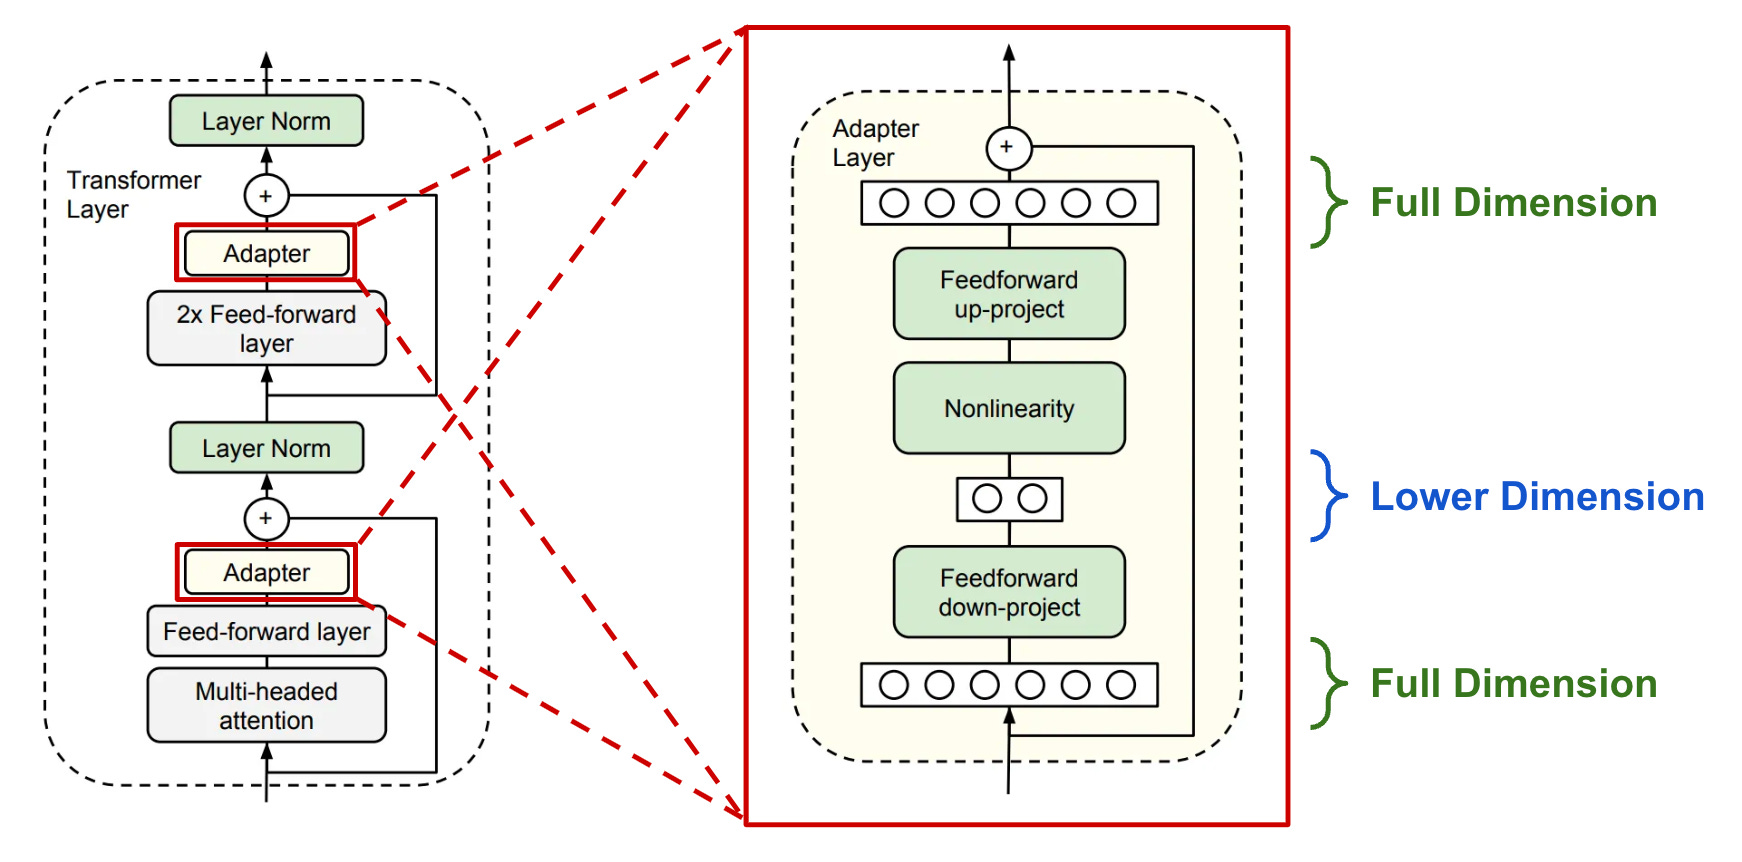
\includegraphics[width=0.9\textwidth]{adapters.jpg}
  \caption{Adapter module integration by Houlsby et al.~\cite{houlsby2019parameter}}
\end{figure}

Low-Rank Adaptation (LoRA) is a PEFT method that introduces low-rank trainable
matrices into the weight structure of a pre-trained model, allowing task-specific adaptation
without updating the full parameter space~\cite{hu2022lora}. Traditional full fine-tuning methods
modify all model weights, which becomes infeasible for large-scale models due to high
memory and storage costs. LoRA addresses this by freezing the original model weights
and learning low-rank decomposition matrices that are injected into specific parts of the
architecture—commonly the query and value projections in the attention mechanism.

LoRA works by expressing the weight update $\Delta W$ as a product of two smaller matrices,
$A \in \mathbb{R}^{d \times r}$ and $B \in \mathbb{R}^{r \times k}$, where $r \ll \min(d, k)$. The modified forward pass becomes:

\begin{equation}
  W x \rightarrow W x + \alpha (AB) x
  \label{lorapass}
\end{equation}

Here, $\alpha$ is a scaling factor (typically a small value like 16 or 32) and $AB$ represents the
trainable rank-$r$ update. This decomposition drastically reduces the number of parameters
introduced during fine-tuning. For instance, instead of learning a $768 \times 768$ matrix (over
half a million parameters), LoRA may only learn a $768 \times 8$ and $8 \times 768$ pair (just over
12K parameters), which is more than 40x fewer parameters.

A key benefit of LoRA is compatibility with pre-trained model checkpoints. Since
LoRA does not alter the base weights, the original model can be shared across tasks,
while task-specific LoRA weights can be stored and applied modularly. This facilitates
multi-task learning, efficient deployment, and on-device adaptation, especially useful in
resource-constrained environments.

LoRA has been widely adopted in modern transformer-based models due to its effectiveness
in low-resource training, and its flexibility makes it suitable for chat models,
instruction tuning, and domain adaptation tasks. Moreover, recent extensions such as
QLoRA further adapt this principle to quantized models, making LoRA viable even in
4-bit or 8-bit precision regimes~\cite{dettmers2023qlora}.

\section{Model Quantization}

Model quantization is a technique used to compress large neural networks by reducing the
precision of the weights and/or activations, which helps in reducing the memory requirements
and improving computational efficiency during inference. Quantization typically
involves converting floating-point numbers, which are 32-bits or 16-bits in standard neural
network implementations, into lower-bit representations, such as 8-bit or even 4-bit
integers. This transformation is important for deploying LLMs in environments with limited
computational resources, such as mobile devices, embedded systems, or GPUs with
limited memory.

The process of quantization generally involves two steps: model weight quantization
(the conversion of model parameters to a lower precision) and activation quantization (the
quantization of intermediate activations during inference). Quantizing both weights and
activations allow the model to run with much lower memory and computational overhead,
but it introduces challenges in maintaining the model's performance and accuracy.

Quantization is especially relevant in the context of PCG and other generative tasks,
where large models are typically required to generate diverse and coherent outputs. By
applying quantization, it is possible to optimize these models for real-time generation
without excessive resource demands.

\subsection{Quantization Techniques (e.g., 4-bit, 8-bit)}

\begin{table}[t]
  \centering
  \scriptsize
  \renewcommand{\arraystretch}{1.3}
  \begin{tabularx}{0.95\textwidth}{
    >{\raggedright\arraybackslash}p{3.5cm}
    >{\centering\arraybackslash}p{3.5cm}
    >{\centering\arraybackslash}p{3cm}
    >{\raggedright\arraybackslash}X
  }
    \toprule
    \textbf{Technique} & \textbf{Memory Reduction} & \textbf{Accuracy Impact} & \textbf{Use Case} \\
    \midrule
    8-bit Quantization & $\sim$4x reduction from FP32 & Low-to-medium & General purpose, widely adopted for LLMs \\
    4-bit Quantization & $\sim$8x reduction from FP32 & High loss & Extremely low-resource environments \\
    \bottomrule
  \end{tabularx}
  \caption{Common quantization methods used to compress and accelerate LLMs}
  \label{table:common_quant}
\end{table}

Quantization techniques can be categorized based on the level of precision and how the
quantization is applied to the model. The most common techniques are 8-bit quantization
and 4-bit quantization, each with its benefits and trade-offs. These techniques are crucial
for reducing the memory footprint of models and enabling efficient deployment in resource-constrained
environments.

8-bit quantization (INT8) is one of the most widely used techniques in model compression.
It reduces the precision of the model's weights and activations to 8 bits, which
is a significant reduction from the typical 32-bit floating-point precision. This technique
is generally effective at achieving a good balance between memory efficiency and model
performance.

4-bit quantization (INT4) reduces the model weights and activations to just 4 bits.
This technique further reduces the memory footprint and computational requirements,
making it particularly useful for extremely resource-constrained devices. However, 4-bit
quantization can introduce significant accuracy loss, and it is often more difficult to
implement without specialized hardware.

The main goal of these quantization techniques is to achieve the best trade-off between
efficiency and accuracy. A summary of the different approaches to model quantization are given in Table~\ref{table:common_quant}.

\subsection{Benefits and Trade-offs}

\begin{table}[t]
  \centering
  \scriptsize
  \renewcommand{\arraystretch}{1.3}
  \begin{tabularx}{0.95\textwidth}{
    >{\raggedright\arraybackslash}p{5cm}
    >{\raggedright\arraybackslash}X
  }
    \toprule
    \textbf{Benefit} & \textbf{Description} \\
    \midrule
    Memory Efficiency & Reduced model size, enabling deployment in resource-limited environments. \\
    Faster Inference & Lower precision enables faster computation, especially on optimized hardware. \\
    Low-Resource Deployment & Makes large models feasible on mobile, embedded, and edge devices. \\
    \bottomrule
  \end{tabularx}
  \caption{Key benefits of applying quantization to language models}
  \label{table:benefits-quant}
\end{table}

\begin{table}[t]
  \centering
  \scriptsize
  \renewcommand{\arraystretch}{1.3}
  \begin{tabularx}{0.95\textwidth}{
    >{\raggedright\arraybackslash}p{5cm}
    >{\raggedright\arraybackslash}X
  }
    \toprule
    \textbf{Trade-off} & \textbf{Description} \\
    \midrule
    Accuracy Loss & Reduced precision can negatively impact generation quality, especially for tasks requiring fine-grained language understanding. \\
    Training Complexity (QAT) & Quantization-aware training can be resource-intensive and time-consuming. \\
    Hardware Dependency & Benefits are dependent on hardware capabilities, which may not support low-precision operations. \\
    \bottomrule
  \end{tabularx}
  \caption{Analysis of trade-offs introduced by model quantization}
  \label{table:trade-offs-quant}
\end{table}

The key benefits of quantization include significant memory savings and faster inference
times, especially when deploying large models for inference in resource-constrained environments.
However, there are trade-offs, particularly with respect to model accuracy.
Quantization tends to introduce some degree of error due to the reduction in precision,
which can affect the generation quality in tasks requiring high accuracy and fluency.
Various benefits and trade-offs of employing model quantization techniques
are listed in Table~\ref{table:benefits-quant} and Table~\ref{table:trade-offs-quant} respectively.

\section{Transformers and Text Generation}

\begin{figure}[t]
  \centering
  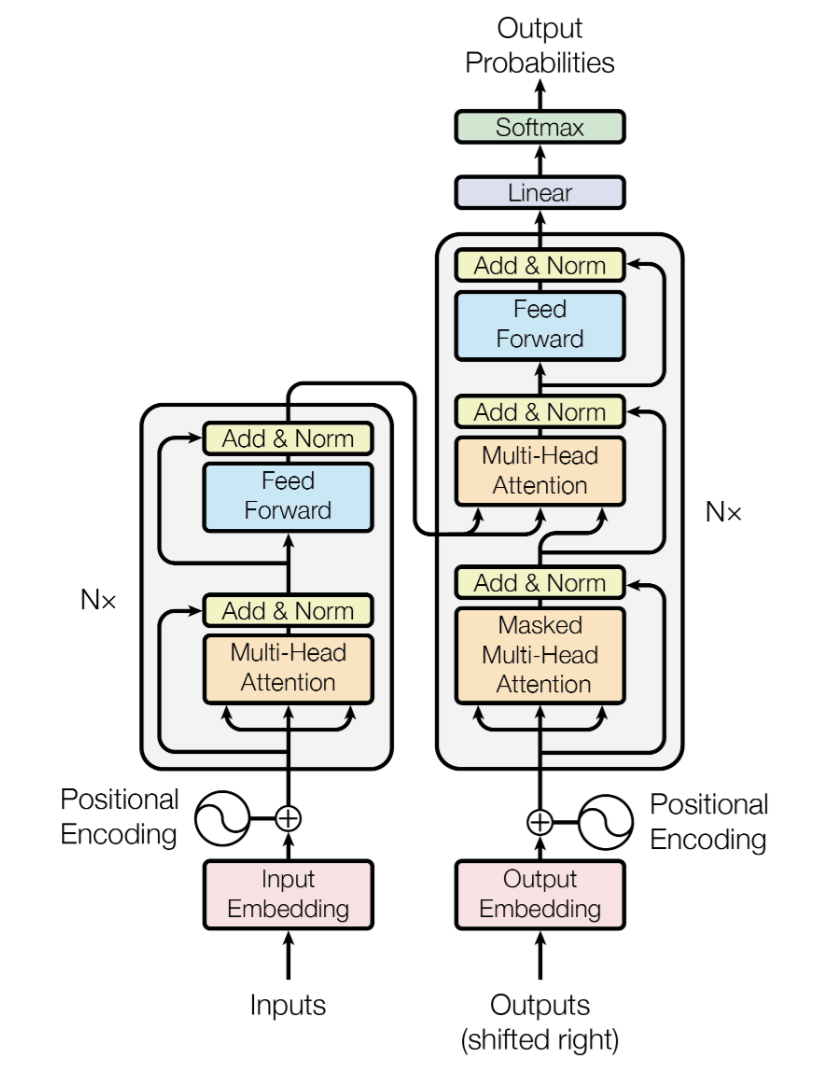
\includegraphics[width=0.5\textwidth]{transformer_architecture.png}
  \caption{Transformer architecture by Vaswani et al.~\cite{vaswani2017attention}}
\end{figure}

\begin{figure}[t]
  \centering
  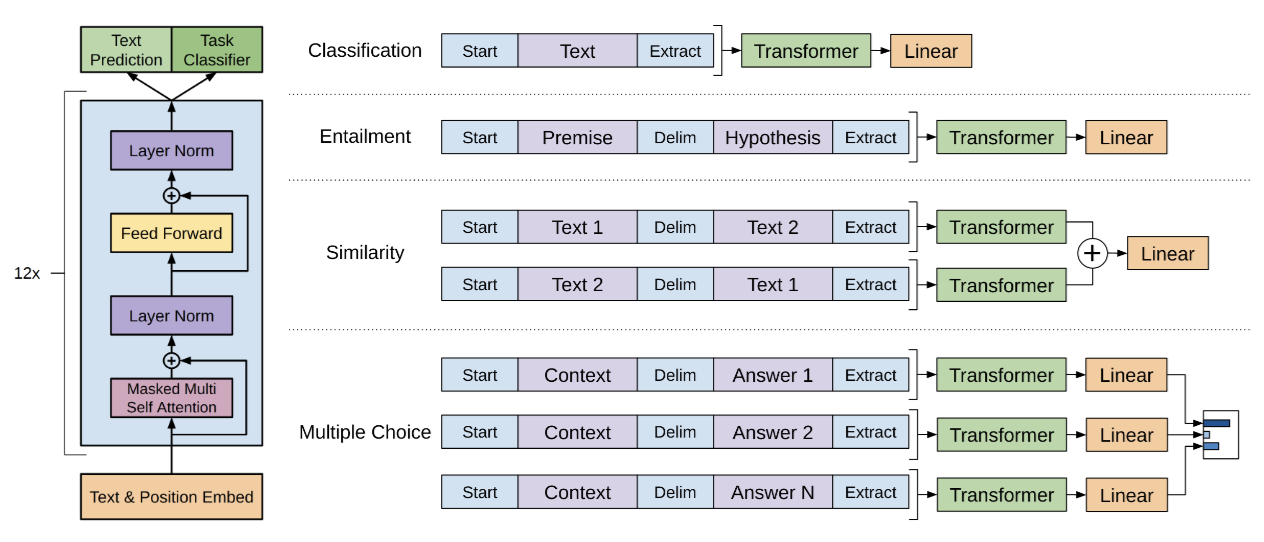
\includegraphics[width=0.9\textwidth]{autoregressive.png}
  \caption{Transformer and autoregressive generation using tokenized inputs and a softmax output layer by Radford et al.~\cite{radford2018improving}}
\end{figure}

Transformer architectures, introduced by Vaswani et al. (2017)~\cite{vaswani2017attention}, revolutionized NLP by
replacing recurrence with attention mechanisms, enabling parallel computation and better
handling of long-range dependencies. The core of the Transformer is the self-attention
mechanism, which allows each token to weigh the importance of other tokens in a sequence
dynamically. This structure significantly improves scalability and representational capacity,
forming the backbone of most modern LLMs.

Transformers consist of stacked encoder and/or decoder layers. For autoregressive text
generation tasks, models typically adopt a decoder-only architecture, as seen in GPT-style
models. These models predict the next token in a sequence based on the previously
generated tokens, learning the conditional probability distribution over sequences as seen
in Equation~\ref{tokengen}.

Each decoder block includes multi-head masked self-attention (to preserve causality),
feed-forward layers, residual connections, and normalization layers (typically LayerNorm).
In the context of text generation, the decoder-only transformer model is trained to minimize
the cross-entropy loss between predicted and actual tokens across large-scale corpora
as seen in Equation~\ref{crossentropy}.

This optimization enables the model to learn language structure, semantics, and context,
empowering it to generate coherent, contextually grounded text. During inference,
greedy decoding, beam search, or sampling-based strategies (e.g., top-k, nucleus sampling)
are employed to generate sequences token by token. The quality of generated text
is influenced by model size, training data diversity, and decoding strategy.

\subsection{Causal Language Modeling}

Causal language modeling (CLM) is the fundamental training paradigm for decoder-only
transformer architectures, where the model is trained to predict the next token in a
sequence based solely on the tokens that precede it. It is termed causal because the self-attention
mechanism is masked such that each token can only attend to earlier positions
in the input sequence, strictly preventing any future context from influencing current
predictions. This autoregressive nature ensures that the generation process proceeds one
token at a time, maintaining a left-to-right structure.

The CLM objective is defined as the maximization of the joint likelihood over a sequence
by decomposing it into a product of conditional probabilities as defined in Equation~\ref{tokengen}.

This modeling approach encourages the network to develop a deep understanding of
linguistic dependencies and long-range structure in text. During training, the model is
optimized using cross-entropy loss, comparing the predicted probability distribution with
the actual next token.

CLM is particularly suited for generative tasks where output sequences must be fluent,
coherent, and sensitive to prior context. It has found significant application in storytelling,
dialogue generation, and PCG for games, where maintaining narrative consistency and
character-specific voice across generated outputs is critical. Moreover, because the model
generates text one token at a time, it is naturally aligned with inference-time decoding
techniques such as greedy decoding, beam search, and sampling, allowing fine-grained
control over generation behavior.

\subsection{Tokenization and Prompt Formats}

Before training or inference, raw text must be tokenized into discrete units understood
by the model. Most transformer-based LLMs use subword tokenization strategies like
byte pair encoding (BPE)~\cite{shibata1999byte}, WordPiece~\cite{song2020fast}, or SentencePiece~\cite{kudo2018sentencepiece}. These techniques
balance vocabulary size with the ability to represent rare or unknown words through compositional
subunits. GPT-2 uses BPE-based tokenization with a vocabulary of $\sim$50,000
tokens, whereas LLaMA models typically use SentencePiece with byte-level fallback for
multilingual robustness.

Prompt formatting plays a crucial role in guiding autoregressive generation. A well-structured
prompt helps align the model's generation behavior with task-specific needs.
For PCG, especially for quests and dialogue, the structured XML-like format we use in
this project provides an explicit and parseable schema that delineates each component of
the generated content, such as \texttt{<|begin\_quest|>}, \texttt{<|objective|>}, \texttt{<|quest\_giver|>}, and
\texttt{<|end\_quest|>}. This format not only improves model interpretability but also ensures
consistency across different samples by providing strong inductive biases during both
training and inference.

By enforcing a rigid prompt structure, we reduce the variability in input-output mappings
and facilitate easier post-processing and validation. Furthermore, the format aids
in fine-tuning and evaluation, allowing automatic extraction of key fields without relying
on fragile heuristics. The inclusion of special tokens and structural boundaries also
conditions the model more effectively, promoting accurate task alignment, especially in
constrained generation scenarios like low-resource training or quantized models.

This approach is particularly beneficial for domain-specific applications such as RPG
quest generation, where narrative components must adhere to recognizable patterns.
Structured prompts help the model disambiguate semantic roles and maintain coherence,
even in zero-shot or few-shot settings.

\section{Procedural Quest Generation}

PQG is the computational process of automatically generating quests (structured narrative
tasks or missions) for players within a digital game environment. Unlike manually
authored quests, which are created by game designers, PQG enables the dynamic and
scalable creation of narrative content through algorithmic methods. The core motivation
behind PQG is to reduce authoring costs, increase content variability, and improve
replayability, especially in open-world or sandbox-style games.

\subsection{Structure and Components of a Quest}

\begin{figure}[t]
  \centering
  \begin{tikzpicture}[
    node distance=2cm,
    component/.style={
      draw, rectangle, rounded corners=5pt,
      minimum width=6cm, minimum height=2cm,
      align=center, fill=#1!30, font=\scriptsize,
      text width=5cm, inner sep=8pt, drop shadow
    },
    arrow/.style={->, thick},
    every node/.style={font=\scriptsize}
  ]
    \node[component=blue] (actors) {
      \textbf{Actors}\\[6pt]
      NPCs provide context and immersion, and deliver dialogue and quests
    };
    \node[component=green, right=of actors] (objectives) {
      \textbf{Objectives}\\[6pt]
      Tasks like fetch, escort, explore, defend that define player goals
    };
    \node[component=orange, below=of objectives] (constraints) {
      \textbf{Constraints}\\[6pt]
      Time, resources, or conditions shape how objectives must be completed
    };
    \node[component=purple, left=of constraints] (rewards) {
      \textbf{Rewards}\\[6pt]
      Experience, items, currency, or story progress as incentives
    };

    \draw[arrow] (actors) -- (objectives);
    \draw[arrow] (objectives) -- (constraints);
    \draw[arrow] (constraints) -- (rewards);
    \draw[arrow] (rewards) -- (actors);
  \end{tikzpicture}
  \caption{Circular flow diagram illustrating the core components of a quest in game design: actors, objectives, constraints, and rewards. Each component plays a critical role in shaping player experience and quest structure.}
  \label{fig:quest-components}
\end{figure}

In game design, a quest refers to a carefully constructed sequence of tasks or challenges
assigned to the player, designed to fulfill a specific in-game objective. Quests are foundational
to many games, especially RPGs, as they provide narrative context, gameplay
direction, and a sense of purpose. They are often embedded with storytelling elements,
gameplay mechanics, and incentive structures, combining to create engaging and meaningful
player experiences.

Quests typically begin with actors, often non-player characters (NPCs), who serve
as quest givers or participants in the unfolding events. These characters help establish the
quest in the game world such that they deliver dialogue, offer context, or accompany
the player on their journey. The interactions of these quest givers with the player reinforce
the immersion within the game's storyline and explain the worldbuilding.

At the core of each quest are the objectives that are the specific tasks the player is
expected to accomplish. These can range from common actions like retrieving a lost item
(“fetch quests”) and guiding a character safely through danger (“escort quests”) to more
dynamic challenges such as defending a location, exploring uncharted areas, or eliminating
threats. Quests often combine multiple objective types in a sequence to form multi-step
missions. This enhances the gameplay complexity and variety.

Quests are further tied to the constraints that influence how objectives must be
achieved. These may include time restrictions, resource limitations, or conditional requirements
for success. For example, a quest may need to be completed before nightfall,
using only a limited set of tools, or without being detected. Such constraints introduce
strategic thinking, increase the difficulty of the gameplay, and differentiate one quest
experience from another.

Upon completion, quests provide rewards as incentives for the player's effort. These
rewards may take various forms, including experience points (EXP) that contribute to
character progression, valuable in-game items, currency, or narrative developments such as
unlocking new characters or advancing the storyline. The reward structure often correlates
with the complexity or risk associated with the quest, reinforcing the player's sense of
accomplishment.

Altogether, these four elements, namely actors, objectives, constraints, and rewards,
constitute the fundamental building blocks of a quest~\cite{howard2022quests}. A deep understanding of these
components is not only vital for traditional quest design but also forms the basis for
automating the generation of quests through procedural methods.

\subsection{Procedural Generation in Quest Design}

\begin{table}[t]
  \centering
  \scriptsize
  \renewcommand{\arraystretch}{1.3}
  \begin{tabularx}{0.95\textwidth}{
    >{\raggedright\arraybackslash}p{2.5cm}
    >{\raggedright\arraybackslash}p{3cm}
    >{\raggedright\arraybackslash}X
    >{\raggedright\arraybackslash}X
    >{\raggedright\arraybackslash}X
  }
    \toprule
    \textbf{Approach} & \textbf{Method Used} & \textbf{Narrative Coherence} & \textbf{Flexibility} & \textbf{Example Systems} \\
    \midrule
    Rule-based & Predefined rules and templates combining structured quest components & Moderate - structured but often lacks narrative depth & Low - limited variation leads to repetition & Classic dungeon crawlers, Skyrim radiant quests~\cite{skyrimradiantquest} \\
    Planning-based & AI planning methods like STRIPS to generate goal-driven quest sequences & High - ensures logical progression and goal alignment & Moderate - adapts to context but constrained by planner limits & STRIPS-based planners~\cite{fikes1971strips}, PaSSAGE~\cite{thue2007interactive} \\
    Grammar-based & Formal grammars and domain-specific ontologies to define quest structure & High - formalizes quest logic and relationships & Moderate - dependent on predefined models and coverage & Mission graph system~\cite{dormans2010adventures}, Doran \& Parberry's quest generator~\cite{doran2011prototype} \\
    Generative models & Data-driven models and LLMs for narrative generation & Very High - produces rich, context-aware stories & High - adaptable to a wide range of themes and player inputs & GPT-based quest generators, AI Dungeon~\cite{ai-dungeon} \\
    \bottomrule
  \end{tabularx}
  \caption{Comparative analysis of common PQG methods}
  \label{table:pqg-approaches}
\end{table}

Procedural generation is a powerful content creation paradigm widely used in video games
to algorithmically produce environments, characters, and other game assets, often enabling
large-scale variability and replayability. PQG extends this concept to the domain
of quest design, aiming to automate the creation of quests that are not only structurally
diverse but also narratively engaging and contextually appropriate within the game world.

Various computational techniques are employed in PQG to achieve this goal. One
common approach is the use of algorithmic rules or templates, which define predefined
structures or patterns that quests can follow. These templates can be customized with
variable content, allowing for a wide range of quest variations while maintaining logical
consistency.

Another technique involves planning algorithms, typically drawn from AI, which simulate
goal-driven behavior by generating sequences of actions that lead from an initial game
state to a desired outcome. This enables the generation of quests that mimic intentionality
and logical progression, often making them feel more believable and purpose-driven.

Grammars and ontologies are also used to formally define the relationships between
quest components such as actions, characters, locations, and objectives. By encoding
domain knowledge into structured formalisms, grammars and ontologies help ensure that
generated quests are semantically coherent and compatible with the broader game world.
Dormans (2010) introduced a grammar-based approach that combines mission structure
and spatial layout generation through graph rewriting techniques, allowing for the creation
of quests that are both logically structured and integrated with the game environment~\cite{dormans2010adventures}.

More recently, machine learning models, particularly LLMs, have been integrated into
PQG systems to enhance narrative richness and human-like expression~\cite{vartinen2022generating}. These models
can generate quest dialogues, descriptions, and plot developments that are contextually
nuanced and linguistically natural, elevating the player's narrative experience.

The overarching objective of PQG is not merely to automate quest production, but
to do so in a manner that maintains narrative coherence, adapts to player behavior,
and aligns with the dynamic context of the game. This makes PQG a challenging yet
promising area of research in PCG, where both design constraints and player engagement
must be carefully balanced.

\newpage
